%%%%%%%%%%%%%%%%%%%%%%%%%%%%%%%%%%%%%%%%%%%%%%%%%%%%%%%%%%%%%%%%%%%%%%
% Lớp 10 | Phương pháp tọa độ trong mặt phẳng (𝑂𝑥𝑦) | Tọa độ của véctơ
% Dạng 0H9?1-3: Tọa độ điểm và véctơ trên hệ  trục Oxy
% Số câu: 40  (sinh tự động bởi tach_cau.py; từ nay thầy sửa trực tiếp file này)
%%%%%%%%%%%%%%%%%%%%%%%%%%%%%%%%%%%%%%%%%%%%%%%%%%%%%%%%%%%%%%%%%%%%%%

%%%%%%%%%%%%%%%% TRẮC NGHIỆM 4 PHƯƠNG ÁN %%%%%%%%%%%%%%%%

% nguồn: MaHoaNH_TracNghiem_Lop10
\begin{ex}%[0H9N1-3]%[ma:3595828b]
	Trong mặt phẳng tọa độ $Oxy$ cho  $A(5; 3)$, $B(7; 8)$. Tìm tọa độ của vectơ $\overrightarrow{AB}$.
	 \choice
		 {$(15; 10)$}
		{\True $(2;  5)$}
		{$(2; 6)$} 
		 {$(-2;-5)$}
	\loigiai{Ta có  $\overrightarrow{AB}=(2; 5)$.}
\end{ex}

% nguồn: MaHoaNH_TracNghiem_Lop10
\begin{ex}%[0H9N1-3]%[ma:327c7103]
	Trong mặt phẳng tọa độ  $Oxy$ cho $A(5; 3)$, $B(7; 8)$. Tọa độ của véctơ $\overrightarrow{AB}$ là
	 \choice
		 {$(-2;-5)$}
		 {$(12; 11)$}
		{\True $(2;  5)$}
		{$(2; 6)$} 
	\loigiai{Ta có $\overrightarrow{AB}=(7-5;  8-3)=(2; 5)$.}
\end{ex}

% nguồn: MaHoaNH_TracNghiem_Lop10
\begin{ex}%[0H9N1-3]%[ma:1fe5a2ff]
	Cho $\overrightarrow{a}=(3;-4)$, $\overrightarrow{b}=(-1; 2)$. Tìm tọa độ  của $\overrightarrow{a}+\overrightarrow{b}$.
	 \choice
		{$(-4;  6)$}
		{\True  $(2;-2)$}
		{$(4;-6)$} 
		{$(-3;-8)$} 
	 \loigiai{
	 Ta có $\overrightarrow{a}+\overrightarrow{b}=(3+(-1);-4+2)=(2;-2)$.}
\end{ex}

% nguồn: MaHoaNH_TracNghiem_Lop10
\begin{ex}%[0H9N1-3]%[ma:b8652759]
	Trong mặt phẳng $Oxy$, cho $A(5; 2)$, $B(10; 8)$. Tọa độ của $\overrightarrow{AB}$ là 
	\choice 
		 {$(2; 4)$}
		{\True $(15; 10)$} 
		 {$(50; 16)$}
		{$(5;  6)$}
	 \loigiai{
		Ta có $A(5; 2)$, $B(10; 8)$  nên $ \overrightarrow{AB} = (15; 10) $.
	} 
\end{ex}

% nguồn: MaHoaNH_TracNghiem_Lop10
\begin{ex}%[0H9N1-3]%[ma:5805c0c0]
	 Cho $\overrightarrow{a}=(3;-4)$. Chọn khẳng định đúng?
	 \choice
		{\True $\overrightarrow{a}=3\overrightarrow{i}-4  \overrightarrow{j}$}
		{$\overrightarrow{a}=-4\overrightarrow{i}+3 \overrightarrow{j}$} 
		 {$\overrightarrow{a}=3\overrightarrow{i}+4 \overrightarrow{j}$}
		 {$\overrightarrow{a}=-3\overrightarrow{i}+4 \overrightarrow{j}$}
	 \loigiai{
		Ta  có $\overrightarrow{a}=(3;-4) \Rightarrow \overrightarrow{a}=3 \overrightarrow{i}-4 \overrightarrow{j}$.
	 }
\end{ex}

% nguồn: MaHoaNH_TracNghiem_Lop10
\begin{ex}%[0H9N1-3]]%[ma:a0eeea45]
	Trong mặt phẳng với hệ trục tọa độ $\left(O;  \overrightarrow{i}; \overrightarrow{j}\right)$ cho điểm $M$ thỏa mãn $\overrightarrow{O M}=-2 \overrightarrow{i}+3 \overrightarrow{j}$. Tọa độ của điểm $M$ là
	 \choice
		{\True  $(-2; 3)$}
		 {$(2;-3)$}
		{$(3;-2)$} 
		 {$(-3; 2)$}
	\loigiai{ 
		$\overrightarrow{O M}=-2 \overrightarrow{i}+3  \overrightarrow{j}$ nên tọa độ điểm $M$ là $(-2; 3)$.
	 }
\end{ex}

% nguồn: MaHoaNH_TracNghiem_Lop10
\begin{ex}%[0H9N1-3]%[ma:f0f1e2ba]
	Cho tam giác  $ABC$ với $A(1;4)$, $B(-2;2)$, $C(4;0)$. Tìm tọa độ $\overrightarrow{AM}$ với $M$ là trung điểm $BC$.
	 \choice
		 {$\overrightarrow{AM}=(-3;0)$}
		 {$\overrightarrow{AM}=(0;3)$}
		{\True  $\overrightarrow{AM}=(0;-3)$}
		 {$\overrightarrow{AM}=(3;0)$}
	 \loigiai{
		Vì $M$  là trung điểm $BC$ nên $\heva{&x_M=\dfrac{x_C+x_B}{2} \\&y_M=\dfrac{y_C+y_B}{2}}\Leftrightarrow \heva{&x_M=1 \\&y_M=1}$.\\
	 Suy ra $\overrightarrow{AM}=(0;-3)$.}
\end{ex}

% nguồn: MaHoaNH_TracNghiem_Lop10
\begin{ex}%[0H9N1-3]%[ma:cea7e83b]
	Trong mặt phẳng $Oxy$, cho hai điểm $A\left(-3;1\right)$ và $B\left(6;5\right)$.  Tìm tọa độ trọng tâm $G$ của tam giác $OAB$ (với $O$ là gốc tọa độ).
	\choice 
		 {$G\left(\dfrac{3}{2};3\right)$}
		 {$G\left(3;\dfrac{4}{3}\right)$}
		{\True  $G\left(1;2\right)$}
		{$G\left(2;1\right)$} 
	\loigiai{ 
	Ta có $\heva{&x_G= \dfrac{0+(-3)+6}{3}=1\\  &y_G= \dfrac{0+1+5}{3}=2}$. Vậy toạ độ $G(1; 2)$.
	} 
\end{ex}

% nguồn: MaHoaNH_TracNghiem_Lop10
\begin{ex}%[0H9N1-3]%[ma:f517df5c]
	Trong mặt phẳng tọa độ $ Oxy $, cho $ A(-1;0) $,  $ B(0;2) $. Véc-tơ $ \overrightarrow{AB} $ có tọa độ là
	 \choice
		{$ (-1;2)  $}
		 {$ (-1;-2) $}
		{\True  $ (1;2) $}
		{$ (1;-2)  $}
	\loigiai{ 
		 Ta có $ \overrightarrow{AB}=(1;2) $.
	} 
\end{ex}

% nguồn: MaHoaNH_TracNghiem_Lop10
\begin{ex}%[0H9N1-3]%[ma:9aad0e67]
	Trong mặt  phẳng $Oxy$, cho $A(5;2)$, $B(10;8)$. Tọa độ véc-tơ $\overrightarrow{AB}$ là
	\choice 
		{$(50;6)$} 
		 {$(15;10)$}
		 {\True $(5;6)$}
		{$(2;4)$} 
	\loigiai{ 
		Tọa độ véc-tơ $\overrightarrow{AB}=(5;6)$. 
	 }
\end{ex}

% nguồn: MaHoaNH_TracNghiem_Lop10
\begin{ex}%[0H9N1-3]%[ma:d3c7f008]
	Trong mặt phẳng với hệ trục tọa độ $Oxy$, cho hai điểm $A(1;2)$, $B(-2;5)$. Tọa độ trung  điểm $I$ của đoạn thẳng $AB$ là
	 \choice
		 {$I(-1;7)$}
		{\True $I\left(-\dfrac{1}{2};\dfrac{7}{2}\right)$} 
		{$I\left(\dfrac{1}{2};-\dfrac{7}{2}\right)$} 
		{$I\left(-\dfrac{1}{2};-\dfrac{7}{2}\right)$} 
	 \loigiai{
		Áp dụng biểu thức tọa độ của của trung điểm, ta  có $\heva{&x_{I}=\dfrac{x_{A}+x_{B}}{2}=-\dfrac{1}{2}\\&y_{I}=\dfrac{y_{A}+y_{B}}{2}=\dfrac{7}{2}.}$\\
		 Vậy tọa độ trung điểm $I$ của đoạn thẳng $AB$ là $I\left(-\dfrac{1}{2};\dfrac{7}{2}\right)$.
	 }
\end{ex}

% nguồn: MaHoaNH_TracNghiem_Lop10
\begin{ex}%[0H9N1-3]%[ma:1924e23c]
	Trong mặt phẳng tọa độ $Oxy$, cho $M(2;4)$  và $N(-6;2)$. Tọa độ trung điểm $I$ của đoạn thẳng $MN$ là
	 \choice
		 {$(4;6)$}
		{$(-4;6)$} 
		 {$(2;3)$}
		{\True $(-2;3)$} 
	\loigiai{ 
		Do $I$ là trung  điểm của đoạn $MN$ nên $x_I=\dfrac{2-6}{2}=-2$; $y_I=\dfrac{4+2}{2}=3$.\\
		Vậy $I(-2;3)$. 
	} 
\end{ex}

% nguồn: MaHoaNH_TracNghiem_Lop10
\begin{ex}%[0H9N1-3]%[ma:42afb354]
	Trong mặt phẳng tọa độ $Oxy$, cho đường thẳng $d \colon 7x+3y-21=0$. Điểm nào sau đây thuộc đường thẳng $d$? 
	 \choice
		 {$D(5;0)$}
		{\True $C(3;0)$} 
		{$B(-3;0)$} 
		{$A(4;0)$} 
	 \loigiai{
		 Với $y=0 \Rightarrow 7x+3 \cdot 0-21=0 \Rightarrow x=\dfrac{21}{7}=3$.\\
		Vậy $C(3;0)$ thuộc đường  thẳng $d$.
	} 
\end{ex}

% nguồn: MaHoaNH_TracNghiem_Lop10
\begin{ex}%[0H9N1-3]%[ma:065fb853]
	Trong mặt phẳng $Oxy$ cho hai điểm $A$, $B$ biết $A(-3;5)$, $B(5;1)$. Tìm tọa độ trung điểm $M$  của đoạn thẳng $AB$.
	\choice 
		 {$(-1;-3)$}
		 {\True $(1;3)$}
		 {$(-1;3)$}
		{$(1;-3)$} 
	 \loigiai{
		Vì $M$  là trung điểm của $AB$ nên ta có
		$\heva{&x_M = \dfrac{x_A+x_B}{2} = \dfrac{-3+5}{2} =  1 \\& y_M = \dfrac{y_A+y_B}{2} = \dfrac{5+1}{2}=3}$.\\
		Vậy  $M(1;3)$.
	 }
\end{ex}

% nguồn: MaHoaNH_TracNghiem_Lop10
\begin{ex}%[0H9N1-3]%[ma:0093c3d4]
	Trong hệ tọa độ $Oxy$, cho $\overrightarrow{u}=\dfrac{1}{2} \overrightarrow{i}-5 \overrightarrow{j}$. Tọa  độ $\overrightarrow{u}$ là
	\choice 
		{$\overrightarrow{u}=\left(\dfrac{1}{2}; 5\right)$} 
		{\True $\overrightarrow{u}=\left(\dfrac{1}{2};-5\right)$} 
		{$\overrightarrow{u}=(-1;  10)$}
		{$\overrightarrow{u}=(1;-10)$} 
	 \loigiai{
		Ta  thấy
		 $$
		\overrightarrow{u}=\dfrac{1}{2} \overrightarrow{i}-5  \overrightarrow{j}
		\Rightarrow 
		\overrightarrow{u}=\left(\dfrac{1}{2};-5\right). 
		 $$
	 }
\end{ex}

% nguồn: MaHoaNH_TracNghiem_Lop10
\begin{ex}%[0H9H1-3]%[ma:96f5d6a0]
	Trong mặt phẳng tọa độ $Oxy$, cho hai điểm $A(-1;6)$ và $B(3;4)$. Tìm tọa độ điểm $M$ là trung điểm của  đoạn thẳng $AB$.
	\choice 
		{$M\left(2;10\right)$} 
		 {$M\left(2;-1\right)$}
		{\True $M\left(1;5\right)$} 
		 {$M\left(4;-2\right)$}
	 \loigiai{
		$M(x;y)$ là trung điểm $AB$ $\Leftrightarrow \heva{&x=\dfrac{-1+3}{2}\\& y=\dfrac{6+4}{2}}\Leftrightarrow \heva{&x=1\\&y=5}\Rightarrow M\left(1;5\right)$. 
	} 
\end{ex}

% nguồn: MaHoaNH_TracNghiem_Lop10
\begin{ex}%[0H9H1-3]%[ma:c2313e59]
	Trong mặt phẳng $Oxy$, cho hình bình hành $ABCD$ biết $A(2; 1)$, $B(2;-1)$, $C(-2;-3)$. Tọa độ giao điểm hai đường chéo của hình bình hành  $ABCD$ là
	\choice 
		 {$(2; 0)$}
		 {$(2; 2)$}
		{$(0;-2)$} 
		{\True $(0;-1)$} 
	\loigiai{ 
		Giao điểm hai đường chéo $ I $ là trung điểm  của $A C$.
		$$ 
		\heva{&x_I = \dfrac{x_A+x_B}{2}=0 \\ &y_I =  \dfrac{y_A+y_B}{2}=-1.}
		$$ 
		Vậy tọa độ giao điểm hai đường  chéo là $I(0;-1)$.
	} 
\end{ex}

% nguồn: MaHoaNH_TracNghiem_Lop10
\begin{ex}%[0H9H1-3]%[ma:5775336e]
	Trong hệ trục tọa độ $Oxy$, cho $A(-4; 1)$, $B(2; 4)$, $C(2;-2)$. Tọa độ  trọng tâm $G$ của tam giác $ABC$ là
	\choice 
		 {$G\left(0; \dfrac{3}{2}\right)$}
		{\True  $G(0; 1)$}
		 {$G(0; 3)$}
		{$G\left(\dfrac{3}{2}; 0\right)$} 
	\loigiai{ 
		$G$ là trọng tâm của  tam giác $ABC$ nên ta có
		$$ 
		\heva{&x_G=\dfrac{-4+2+2}{3}=0  \\ &y_G=\dfrac{1+4-2}{3}=1.}
		 $$
		 Vậy $G(0; 1)$.
	} 
\end{ex}

% nguồn: MaHoaNH_TracNghiem_Lop10
\begin{ex}%[0H9H1-3]%[ma:dbca912b]
	Trong mặt phẳng toạ độ $Oxy$,  cho hai điểm $A(1;-3)$, $B(3; 1)$. Toạ độ trung điểm $I$ của đoạn thẳng $AB$ là
	 \choice
		{$I(-1;-2)$} 
		{\True $I(2;-1)$} 
		 {$I(1;-2)$}
		{$I(2; 1)$} 
	\loigiai{ 
		Toạ  độ trung điểm $I$ của đoạn thẳng $AB$ là
		 $$
		\heva{&x_I = \dfrac{x_A+x_B}{2}=2 \\ &y_I = \dfrac{y_A+y_B}{2}=-1.} 
		 $$
		 Vậy $I(2;-1)$.
	 }
\end{ex}

% nguồn: MaHoaNH_TracNghiem_Lop10
\begin{ex}%[0H9H1-3]%[ma:41a954dd]
	Trong hệ tọa độ $Oxy$, cho tam giác $ABC$ có $A(6; 1)$, $B(-3; 5)$ và trọng tâm $G(-1; 1)$. Tìm tọa  độ đỉnh $C$.
	 \choice
		 {$C(6;-3)$}
		 {$C(-6; 3)$}
		 {\True $C(-6;-3)$}
		 {$C(-3; 6)$}
	 \loigiai{
		 Gọi $C(x; y)$. Vì $G$ là trọng tâm tam giác $ABC$ nên
		$$ 
		 \heva{&\dfrac{6+(-3)+x}{3}=-1 \\ &\dfrac{1+5+y}{3}=1}
		 \Leftrightarrow
		 \heva{&x=-6 \\ &y=-3.}
		$$ 
	} 
\end{ex}

% nguồn: MaHoaNH_TracNghiem_Lop10
\begin{ex}%[0H9H1-3]%[ma:8e605c9e]
	Trong mặt phẳng  $Oxy$ cho $A(-2; 0)$, $B(5;-4)$. Tọa độ điểm $E$ đối xứng với $A$ qua $B$ là
	 \choice
		{$E(-9; 4)$} 
		{$E(12;  8)$}
		{\True  $E(12;-8)$}
		 {$E(-8; 12)$}
	 \loigiai{
		Điểm $E$ đối xứng với $A$ qua $B$ nên $B$  là trung điểm của đoạn $A E$.
		 Do đó
		 $$
		\heva{&x_E=2 x_B-x_A=2 \cdot 5-(-2)=12;  \quad
		\\ &y_E=2  y_B-y_A=2 \cdot (-4)-0=-8.}
		$$ 
		Vậy $ E(12;-8)  $.
	 }
\end{ex}

% nguồn: MaHoaNH_TracNghiem_Lop10
\begin{ex}%[0H9H1-3]%[ma:4edef424]
	Cho tam giác $ABC$ cân tại $A$ có $B(2;-3)$. Đường cao kẻ từ $A$ cắt cạnh  $BC$ tại điểm $D(-1;3)$. Tọa độ của điểm $C$ là
	\choice 
		 {\True $(-4;9)$}
		 {$(-8;9)$}
		{$(-2;3)$} 
		 {$(-4;8)$}
	 \loigiai{
	\immini{Ta  có $D$ là trung điểm của $BC$.
		$$\heva{&x_D=\dfrac{x_B+x_C}{2}\\&y_D=\dfrac{y_B+y_C}{2}}\Rightarrow\heva{&x_C=2\cdot(-1)-2=-4\\&y_C=2\cdot3+3=9.}$$ 
		Vậy $C(-4;9)$. 
		}{ 
		\begin{tikzpicture}[>=stealth,line join=round,line cap=round,font= \footnotesize,scale=1]
				\path 
					(0,0) coordinate  (B)
					(2,0)  coordinate (C)
					($(B)!0.5!(C)$) coordinate  (D)
					($(D)!1.2!90:(C)$) coordinate (A); 
				\draw (A)--(B)--(C)--(A)  --(D);
				\draw pic [draw,angle radius=2mm]  {right angle =C--D--A};
				 \foreach \x/\g in {A/90,B/180,C/0,D/-90}
				\fill (\x) circle (1pt) 
					($(\x)+(\g:3mm)$) node{$\x$}; 
			\end{tikzpicture}
		} 
	} 
\end{ex}

% nguồn: MaHoaNH_TracNghiem_Lop10
\begin{ex}%[0H9V1-3]%[ma:f32bcf4f]
	Trong mặt phẳng $Oxy$, cho các điểm  $A(-2;1)$, $B(4;0)$, $C(2;3)$. Tìm điểm $M$ biết rằng $\overrightarrow{CM}+3\overrightarrow{AC}=2\overrightarrow{AB}$.
	\choice 
		{\True $M(2;-5)$} 
		{$M(5;-2)$} 
		{$M(-5;2)$} 
		{$M(2;5)$} 
	\loigiai{ 
		Gọi điểm $M(x;y)$. Khi đó ta  có $\overrightarrow{CM}=(x-2;y-3)$, $\overrightarrow{AC}=(4;2)$, $\overrightarrow{AB}=(6;-1)$.\\
		Theo giả thiết ta có $\overrightarrow{CM}+3\overrightarrow{AC}=2\overrightarrow{AB}\Leftrightarrow \heva{&x-2+3\cdot 4=2\cdot 6 \\&y-3+3\cdot 2=2\cdot (-1)}\Leftrightarrow  \heva{&x=2 \\&y=-5.}$\\
	Vậy $M(2;-5)$.} 
\end{ex}

% nguồn: MaHoaNH_TracNghiem_Lop10
\begin{ex}%[0H9V1-3]%[ma:ebf3fbf9]
	Trong hệ  tọa độ $Oxy$, cho tam giác $ABC$ có $B(9; 7)$, $C(11;-1)$. Gọi $M, N$ lần lượt là trung điểm của $AB$, $A C$. Tìm tọa độ của $\overrightarrow{M N}$.
	 \choice
		 {$\overrightarrow{M N}=(2;-8)$}
		{\True  $\overrightarrow{M N}=(1;-4)$}
		{$\overrightarrow{M  N}=(10; 6)$}
		{$\overrightarrow{M  N}=(5; 3)$}
	\loigiai{ 
		Dễ thấy $ MN $ là đường trung bình của tam giác  $ ABC $ mà
		 $$
		\overrightarrow{B C}=(2;-8) \quad  \text{nên} \quad
		\overrightarrow{M N}=\dfrac{1}{2} \overrightarrow{B  C}=(1;-4).
		 $$
	 }
\end{ex}

% nguồn: MaHoaNH_TracNghiem_Lop10
\begin{ex}%[0H9V1-3]%[ma:322aab4b]
	Trong hệ tọa độ $Oxy$, cho tam giác $ABC$ có $C(-2;-4)$, trọng tâm $G(0; 4)$ và trung điểm cạnh $B C$ là $M(2; 0)$. Tổng hoành độ của hai  điểm $A$ và $B$ là
	\choice 
		{$  -2 $}
		{\True $ 2 $} 
		{$ 4 $} 
		{$  8 $}
	\loigiai{ 
		Vì $M$ là trung điểm $B C$  nên
		$$ 
		\heva{&x_B=2 x_M-x_C=2.2-(-2)=6 \\  &y_B=2 y_M-y_C=2.0-(-4)=4}
		\Rightarrow  B(6; 4).
		$$ 
		 Vì $G$ là trọng tâm tam giác $ABC$ nên
		 $$
		\heva{&x_A=3 x_G-x_B-x_C=-4 \\ &y_A=3 y_G-y_B-y_C=12} 
		\Rightarrow A(-4;  12).
		$$ 
		Suy ra  $x_A+x_B=2$.
	 }
\end{ex}

% nguồn: MaHoaNH_TracNghiem_Lop10
\begin{ex}%[0H9V1-3]%[ma:28b8203e]
	Trong hệ tọa độ  $Oxy$, cho $A(1; 3)$, $B(4; 0)$, $C(2;-5)$. Tìm tọa độ điểm $M$ thỏa mãn hệ thức $\overrightarrow{M A}+\overrightarrow{M B}-3 \overrightarrow{M C}=\overrightarrow{0}$?
	\choice 
		{$M(1; 18)$} 
		 {$M(-1; 18)$}
		 {\True $M(1;-18)$}
		{$M(-18; 1)$} 
	 \loigiai{
		 Gọi tọa độ $M(x; y)$.
		\\ 
		Suy ra $\overrightarrow{M A}=(1-x; 3-y)$, $\overrightarrow{M B}=(4-x;-y)$, $\overrightarrow{M C}=(2-x;-5-y)$. 
		 \\
		Ta có 
		$$ 
		\overrightarrow{M A}+\overrightarrow{M B}-3 \overrightarrow{M C}=\overrightarrow{0} 
		\Leftrightarrow 
		\heva{&(1-x)+(4-x)-3(2-x)=0 \\ &3-y-y-3(-5-y)=0} 
		\Leftrightarrow 
		\heva{&x=1 \\  &y=-18.}
		$$ 
	 }
\end{ex}

% nguồn: MaHoaNH_TracNghiem_Lop10
\begin{ex}%[0H9C1-3]%[ma:44c4be5f]
	Cho ba điểm $A(1;0)$, $B(0;3)$, $C(-3;-5)$. Điểm $M$ thuộc  $Ox$ sao cho $\left| 2\overrightarrow{MA}-3\overrightarrow{MB}+2\overrightarrow{MC}\right|$ bé nhất. Khi đó tọa độ $M$ là
	\choice 
		{$(-3;0)$} 
		 {$(3;0)$}
		 {\True $(-4;0)$}
		{$(4;0)$} 
	 \loigiai{
		 $M\in Ox\Rightarrow M(x;0)$.\\
		Ta có $2\overrightarrow{MA}=(2-2x;0)$, $3\overrightarrow{MB}=(-3x;9)$, $2\overrightarrow{MC}=(-6-2x;-10)$.\\ 
		Suy ra  $2\overrightarrow{MA}-3\overrightarrow{MB}+2\overrightarrow{MC}=(-x-4;-19)$\\
		$\Rightarrow \left| 2\overrightarrow{MA}-3\overrightarrow{MB}+2\overrightarrow{MC}\right|=\sqrt{(x+4)^2+19^2}\ge 19$.\\ 
		Giá trị nhỏ nhất của $\left| 2\overrightarrow{MA}-3\overrightarrow{MB}+2\overrightarrow{MC}\right|$ bằng $19$, dấu  \lq\lq$=$\rq\rq~ xảy ra khi $x=-4$.\\
	Vậy  $M(-4;0)$.}
\end{ex}


%%%%%%%%%%%%%%%% ĐÚNG/SAI %%%%%%%%%%%%%%%%

% nguồn: MaHoaNH_DungSai_Lop10
\begin{ex}%[0H9N1-3]%[ma:801d287c]
	Trong mặt  phẳng tọa độ $Oxy$, cho $A(-2;1)$, $B(1;-3)$, $C(0;1)$. Mỗi khẳng định dưới
	 đây là đúng hay sai?
	\choiceTF 
		{\True Tọa  độ của véc-tơ $\overrightarrow{AB}=(3;-4)$}
		{Tọa độ  của véc-tơ $\overrightarrow{AA}=(-3;4)$}
		{\True  Tọa độ của véc-tơ $\overrightarrow{BC}=(-1;4)$}
		{Tọa  độ của véc-tơ $\overrightarrow{AC}=(-1;-4)$}
	 \loigiai{
		\begin{itemchoice}
			\itemch  Tọa độ của véc-tơ $\overrightarrow{AB}=(3;-4)$.
			\itemch  Tọa độ của véc-tơ $\overrightarrow{AA}=(0;0)$.
			\itemch Tọa độ của  véc-tơ $\overrightarrow{BC}=(-1;4)$.
			\itemch Tọa độ của véc-tơ  $\overrightarrow{AC}=(2;0)$.
		\end{itemchoice}
	} 
\end{ex}

% nguồn: MaHoaNH_DungSai_Lop10
\begin{ex}%[0H9N1-3]%[ma:44e2ba9a]
	Trong mặt phẳng tọa độ $Oxy$, cho $A(1;1)$, $B(2;2)$, $C(3;3)$.  Mỗi khẳng định dưới
	đây là đúng  hay sai?
	\choiceTF 
		{\True Tồn tại điểm $M$  thỏa mãn $\overrightarrow{AM}=(1;1)$}
		 {Tồn tại điểm $N$ thỏa mãn $\overrightarrow{NN}=(1;1)$}
		{\True Tồn tại  điểm $P$ thỏa mãn $\overrightarrow{BP}=(1;1)$}
		{Tồn tại điểm $Q$  thỏa mãn $\overrightarrow{AC}=\overrightarrow{QQ}$}
	 \loigiai{
		\begin{itemchoice}
			\itemch $\overrightarrow{AB}=(1;1)$ nên $\overrightarrow{AM}=\overrightarrow{AB}$. Vậy $M$ trùng $B$. 
			\itemch $\overrightarrow{NN}=(0;0)$. Vậy không tồn tại $N$ thỏa mãn yêu cầu bài  toán.
			 \itemch
			$\overrightarrow{BC}=(1;1)$ nên $\overrightarrow{BP}=\overrightarrow{BC}$. Vậy $P$ trùng  $C$.
			 \itemch
			$\overrightarrow{AC}=(2;2)$ và $\overrightarrow{QQ}=(0;0)$. Vậy  không tồn tại $Q$ thỏa mãn yêu cầu bài toán.
		\end{itemchoice}
	 }
\end{ex}

% nguồn: MaHoaNH_DungSai_Lop10
\begin{ex}%[0H9H1-3]%[ma:03532674]
	Trong mặt phẳng $Oxy$, cho $\vec{OM}=2\vec{i}-\vec{j}$ và  hai điểm $N(1;10)$, $P(3;6)$.
	\choiceTF 
		{\True  $M(2;-1)$}
		 {$MNPQ$ là hình bình hành nếu $Q(-5;16)$}
		{\True $I(2;8)$ là trung điểm  $NP$}
		 {$3\vec{MN}-2\vec{NP}=(-7;27)$}
	 \loigiai{
		\begin{itemchoice}
			\itemch \textbf{Đúng}.\\ 
			$\vec{OM}=2\vec{i}-\vec{j}\Rightarrow M(2;-1)$ 
			\itemch \textbf{Sai}.  \\
			$MNPQ$ là hình bình hành $\Leftrightarrow \vec{MN}=\vec{QP} \Leftrightarrow \heva{&1-2=3-x_Q \\ &10+1=6-y_Q} \Leftrightarrow\heva{&x_Q=4 \\ &y_Q=-5}$ 
			\itemch \textbf{Đúng}.\\ 
			$I$ là trung điểm $NP\Rightarrow  I(2;8).$
			\itemch \textbf{Sai}.  \\
			 $\vec{MN}=(-1;11)$ và $\vec{NP}=(2;-4)$ nên $3\vec{MN}-2\vec{NP}=(-7;41)$.
		\end{itemchoice}
	 }
\end{ex}

% nguồn: MaHoaNH_DungSai_Lop10
\begin{ex}%[0H9V1-3]%[ma:48cefb62]
	Cho $ \overrightarrow{a}=3 \overrightarrow{i}+\overrightarrow{j}  $, $ \overrightarrow{b}=-2 \overrightarrow{j} $. Khi đó
	 \choiceTF
		 {$ \overrightarrow{a}=(-3; 1) $}
		 {\True $ \overrightarrow{b}=(0;-2) $}
		 {$ \overrightarrow{a}+\overrightarrow{b}=(3; 1) $}
		{$ \overrightarrow{a}-\overrightarrow{b}=(3;-3)  $}
	\loigiai{ 
		\begin{itemchoice}
			\itemch Sai.  Ta có $ \overrightarrow{a}=(3; 1) $.
			\itemch Đúng. Ta  có $ \overrightarrow{b}=(0;-2) $.
			\itemch  Sai. Ta có $ \overrightarrow{a}+\overrightarrow{b}=(3; 1)+(0;-2)=(3;-1) $.
			\itemch Sai.  Ta có $ \overrightarrow{a}-\overrightarrow{b}=(3; 1)-(0;-2)=(3; 3) $.
		\end{itemchoice}
	 }
\end{ex}

% nguồn: MaHoaNH_DungSai_Lop10
\begin{ex}%[0H9V1-3]%[ma:f14188d9]
	Trong mặt phẳng toạ độ $ Oxy $, cho $ A(-2; 5) $, $ B(-4;-2) $, $ C(1; 5) $.  Khi đó
	\choiceTF 
		{\True Ba điểm $A, B, C$  không thẳng hàng}
		{\True $G\left(-\dfrac{5}{3}; \dfrac{8}{3}\right)$ là tọa độ trọng tâm của tam  giác $ABC$}
		{Tứ giác $ABCD$ là hình bình hành khi đó tọa độ điểm $D$ là $D(3;  10)$}
		{$ \widehat{A C B}=45^{\circ} $} 
	\loigiai{ 
		\begin{itemchoice}
			 \itemch Đúng.\\
			Ta có  $\overrightarrow{AB}=(-2;-7)$, $\overrightarrow{A C}=(3; 0)$.
			 \\
			Do $\dfrac{3}{-2} \neq \dfrac{0}{-7}$ nên $\overrightarrow{AB}$, $\overrightarrow{A C}$  không cùng phương. Vì vậy ba điểm $A, B, C$ không thẳng hàng.
			\itemch  Đúng.\\
			Do $ G $ là trọng tâm của tam giác $ ABC $ nên tọa độ $ G $  là
			$$ 
			\heva{&x_G = \dfrac{x_A+x_B+x_C}{3} = -\dfrac{5}{3}  \\ &y_G = \dfrac{y_A+y_B+y_C}{3} = \dfrac{8}{3}}.
			 $$
			Vậy $  G\left(-\dfrac{5}{3}; \dfrac{8}{3}\right) $.
			 \itemch Sai.\\
			Giả sử $D(x; y)$.  Ta có $\overrightarrow{AB}=(-2;-7)$, $\overrightarrow{DC}=(1-x; 5-y)$.
			\\ 
			Tứ giác $ABCD$ là hình bình hành nếu 
			 $$
			 \overrightarrow{AB}=\overrightarrow{DC}
			\Leftrightarrow 
			\heva{&-2=1-x  \\ &-7=5-y}
			\Leftrightarrow 
			\heva{&x=3 \\  &y=12.}
			 $$
			Vậy $D(3; 12)$. 
			 \itemch Sai.\\
			Ta  có
			\begin{align*}
				 &AB=\sqrt{(-2)^2+(-7)^2}=\sqrt{53}, \\
				&AC=\sqrt{[1-(-2)]^2+(5-5)^2}=3. 
			\end{align*}
			 Ta có
			 $$
			 \overrightarrow{CA} \cdot \overrightarrow{CB}=(-3) \cdot (-5) + 0 \cdot (-7)=15.
			 $$
			Suy  ra
			 $$
			\cos \widehat{ACB}=\cos \left(\overrightarrow{CA} ,  \overrightarrow{CB}\right)
			=\dfrac{\overrightarrow{CA} \cdot \overrightarrow{CB}}{|\overrightarrow{CA}| \cdot|\overrightarrow{CB}|} 
			=\dfrac{15}{3 \cdot  \sqrt{74}}
			 =\dfrac{5}{\sqrt{74}}.
			 $$
			nên $\widehat{ACB}  \approx 54^{\circ}$.
		\end{itemchoice}
	 }
\end{ex}


%%%%%%%%%%%%%%%% TRẢ LỜI NGẮN %%%%%%%%%%%%%%%%

% nguồn: MaHoaNH_TraLoiNgan_Lop10
\begin{bt}%[0H9H1-3]%[ma:6823de12]
	Trong mặt phẳng tọa độ $Oxy$, cho ba điểm $M(1;-2)$, $N(3;1)$, $P(5;2)$. Điểm $Q(a;b)$ là điểm sao cho tứ giác $MPNQ$ là hình thang cân với hai đáy là $MP$  và $NQ$. Tính tổng $a+b$.
	\shortans{2} 
	 \loigiai{
		Gọi $Q(a;b)$ là điểm sao cho tứ giác $MPNQ$  là hình thang cân.\\
		+ Ta có $\overrightarrow{MP}=(4;4)$; $\overrightarrow{QN}=(3-a;1-b)$.  Vì $\overrightarrow{MP}$ và $\overrightarrow{QN}$ cùng hướng nên
		\[\dfrac{3-a}{4}=\dfrac{1-b}{4}=k>0\Rightarrow 3-a=1-b\Leftrightarrow b=a-2.\quad (1)\]\\ 
		+ Vì  $MQ=NP$ nên ta có
		\[(a-1)^2+(b+2)^2=(5-3)^2+(2-1)^2.\quad  (2)\]
		Thay $(1)$ vào  $(2)$ ta được
		 \[a^2-2a+1+a^2=5\Leftrightarrow 2a^2-2a-4=0\Leftrightarrow \hoac{&a=-1\\&a=2.}\]
		Với $a=-1\Rightarrow b=-3\Rightarrow Q(-1;-3)$.  Lúc này $\overrightarrow{MP}=\overrightarrow{QN}=(4;4)$ nên $MPNQ$ là hình bình hành. Loại trường hợp này.\\
		Với $a=2\Rightarrow b=0\Rightarrow Q(2;0)$. Lúc  này $\overrightarrow{QN}=(1;1)$ cùng hướng với $\overrightarrow{MP}$. Do đó $MPNQ$ là hình thang cân.\\
		Vậy $Q(2;0)$  là điểm cần tìm.
	 }
\end{bt}

% nguồn: MaHoaNH_TraLoiNgan_Lop10
\begin{bt}%[0H9H1-3]%[ma:347d075e]
	Trong  mặt phẳng toạ độ $Oxy$, cho $A(2; 2)$, $B(1;-3)$, $C(-3; 0)$. Điểm $E$ thoả mãn $\overrightarrow{A E}=-2 \overrightarrow{AB}+3 \overrightarrow{A C}$. Khi đó giá trị của $ x_E \cdot y_E $ là bao nhiêu?
	 \shortans{-66}
	\loigiai{ 
		Giả sử $E(x;  y)$.
		Ta  có
		 $$
		 \overrightarrow{A E}=(x-2; y-2), \quad
		\overrightarrow{AB}=(-1;-5),  \quad
		 \overrightarrow{A C}=(-5;-2).
		$$ 
		Suy  ra
		 $$
		-2 \overrightarrow{AB}+3 \overrightarrow{A  C}=(-13; 4).
		 $$
		 Do đó
		 $$
		\overrightarrow{A E}=-2 \overrightarrow{AB}+3 \overrightarrow{A C} 
		\Leftrightarrow 
		\heva{&x-2=-13 \\ &y-2=4} 
		\Leftrightarrow 
		\heva{&x=-11 \\  &y=6.}
		 $$
		 Vậy $x_E \cdot y_E = -66$.
	 }
\end{bt}

% nguồn: MaHoaNH_TraLoiNgan_Lop10
\begin{bt}%[0H9V1-3]%[ma:bde47f50]
	Trong mặt phẳng toạ độ $Oxy$, cho hai điểm $A(1; 5)$, $B(9; 3)$. Điểm $M$ thuộc trục hoành sao cho $\widehat{A M B}=90^{\circ}$. Có bao nhiêu điểm $ M $ thỏa mãn yêu  cầu bài toán?
	\shortans{2} 
	 \loigiai{
		Điểm $M$ thuộc  trục hoành nên giả sử $M(m; 0)$.\\
		Ta có $\overrightarrow{M A}=(1-m; 5)$  và $\overrightarrow{M B}=(9-m; 3)$.\\
		 Theo đề bài
		$$ 
		\widehat{A M  B}=90^{\circ}
		\Leftrightarrow 
		\overrightarrow{M A}  \cdot \overrightarrow{M B}=0
		\Leftrightarrow(1-m)(9-m)+5  \cdot 3=0
		 \Leftrightarrow m^2-10 m+24=0
		 \Leftrightarrow
		\hoac{&m=6 \\ &m=4.} 
		 $$
		Vậy có $ 2 $ trường hợp điểm $M$ thỏa mãn bài toán là $M(4; 0)$ và $M(6;  0)$.
	} 
\end{bt}

% nguồn: MaHoaNH_TraLoiNgan_Lop10
\begin{bt}%[0H9V1-3]%[ma:ecb2c74f]
	Trong mặt phẳng tọa độ $Oxy$, cho hai điểm $M(5; 3)$, $N(-3; 5)$. Điểm $P$ nằm trên trục hoành sao  cho ba điểm $M, N, P$ thẳng hàng. Hoành độ điểm $ P $ là bao nhiêu?
	\shortans{17} 
	\loigiai{ 
		$P$ là điểm  nằm trên trục hoành nên $P(x;0)$.
		 \\
		Ta có  $\overrightarrow{M N}=(-8; 2); \overrightarrow{M P}=(x-5;-3)$.
		\\ 
		Ba điểm $M, N,  P$ thẳng hàng khi
		 $$
		\overrightarrow{M P}=k  \overrightarrow{M N}
		\Leftrightarrow 
		\heva{&x-5=k \cdot(-8)  \\ &-3=k \cdot 2}
		 \Leftrightarrow
		\heva{&x=17 \\ &k=-\dfrac{3}{2}.} 
		 $$
		 Vậy $x_P=17$.
	 }
\end{bt}


%%%%%%%%%%%%%%%% TỰ LUẬN %%%%%%%%%%%%%%%%

% nguồn: MaHoaNH_TuLuan_Lop10
\begin{bt}%[0H9H1-3]%[ma:fc07e4aa]
	Cho hình thang cân $ABCD$ với $A(2; 0)$, $B(0;  2)$, $C(0; 7)$, $D(a;b)$. Tìm giá trị nhỏ nhất của $a+b$.
	 \loigiai{
		Gọi $D(x;  y)$ suy ra $\overrightarrow{CD}=(x;y-7)$, $\overrightarrow{AD}=(x-2;y)$.\\
		$\overrightarrow{AB}=(-2;2)\Rightarrow  AB=2\sqrt{2}$, $\overrightarrow{BC}=(0;5)\Rightarrow BC=5$.
		\begin{center}
			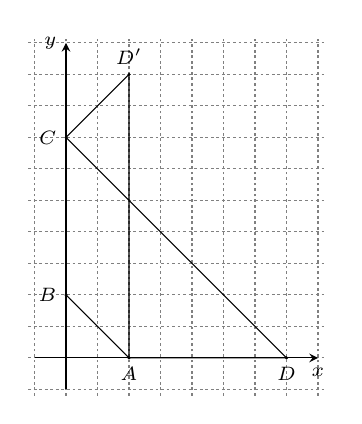
\begin{tikzpicture}[>=stealth,x=1cm,y=1cm,scale=0.4]
					 \def\a{-2}
					 \def\b{3}
					\draw[color=gray,dash pattern=on 1pt  off 1pt,xstep=1.0cm,ystep=1.0cm] (-1.2,-1.2) grid (8.2,10.2);
					\draw[->] (-1,0) -- (8,0) node[below] {\scriptsize  $x$};
					\draw[->] (0,-1) -- (0,10)  node[left] {\scriptsize $y$};
					\coordinate[label=below:\scriptsize $A$] (A) at (2,0); 
					\coordinate[label=left:\scriptsize $B$] (B)  at (0,2);
					\coordinate[label=left:\scriptsize $C$] (C) at  (0,7);
					\coordinate[label=below:\scriptsize $D$] (D) at (7,0); 
					 \coordinate[label=above:\scriptsize $D'$] (D') at (2,9);
					\draw (A)--(B)--(C)--(D)--(A) 
						 (A)--(B)--(C)--(D')--(A);
					\foreach \diem in {A,B,C,D,D'}\fill (\diem)  circle (1.5pt);
				\end{tikzpicture}
		\end{center}
		Trường hợp 1: Hình thang có hai  đáy $A B$, $C D$.\\
		Ta có $\heva{&\overrightarrow{AB},\overrightarrow{CD}\text{  cùng phương}\\&AD=BC}\Leftrightarrow\heva{&\dfrac{x}{-2}=\dfrac{y-7}{2} \\&\sqrt{(x-2)^2+y^2}=5} \Leftrightarrow\heva{&x=-y+7 \\&(-y+7-2)^2+y^2=25}$\\
		$\Leftrightarrow\heva{&x=-y+7 \\&2 y^2-10 y+25=25} \Leftrightarrow\heva{&x=7 \\&y=0} \ \text{hoặc}\ \heva{&x=2 \\&y=5.}$\\ 
		Với $\heva{&x=7 \\&y=0}$ thì  $CD=\sqrt{7^2+(0-7)^2}=7 \sqrt{2} \neq AB$ nên $D(7; 0)$ thỏa mãn.\\
		Với $\heva{&x=2 \\&y=5}$ thì $CD=\sqrt{2^2+(5-7)^2}=2 \sqrt{2}=AB$  (loại).\\
		Trường  hợp 2: Hình thang có hai đáy $BC$, $AD$.\\
		Ta có  $\heva{&\overrightarrow{BC},\overrightarrow{AD}\text{ cùng phương}\\&AB=CD}\Leftrightarrow\heva{&\dfrac{0}{x-2}=\dfrac{5}{y} \\&2\sqrt{2}=\sqrt{x^2+(y-7)^2}} \Leftrightarrow\heva{&\dfrac{x-2}{y}=\dfrac{0}{5} \\&x^2+(y-7)^2=8}$\\
		$\Leftrightarrow\heva{&x=2 \\&(y-7)^2=4} \Leftrightarrow\heva{&x=2 \\&y=5} \ \text{hoặc}\  \heva{&x=2 \\&y=9.}$\\
		 Với $\heva{&x=2 \\&y=9}$ thì $AD=\sqrt{0^2+9^2}=9 \neq BC$ nên $D(2;9)$ thỏa mãn.\\
		Với $\heva{&x=2  \\&y=5}$ thì $AD=\sqrt{0^2+5^2}=5=BC$ (loại).\\
		Vậy giá trị nhỏ nhất của  $a+b$ là $7$.
	 }
\end{bt}

% nguồn: MaHoaNH_TuLuan_Lop10
\begin{bt}%[0H9V1-3]%[ma:27fd36ad]
	Trong  mặt phẳng toạ độ $Oxy$, cho hai điểm $A(4;-2)$ và $B(10; 4)$. Điểm $M$ trên trục tung sao cho $\left|\overrightarrow{M A}+\overrightarrow{M B}\right|$ đạt giá trị nhỏ nhất. Tung độ của điểm $ M $ có giá trị bao nhiêu?
	 \loigiai{
		Điểm $M$ thuộc trục tung nên giả sử $M(0;  m)$.\\
		Ta có $\overrightarrow{M A}=(4;-2-m)$, $\overrightarrow{M B}=(10;4-m)$.\\ 
		Suy ra $\overrightarrow{M A}+\overrightarrow{M  B}=(14; 2-2 m)$.\\
		Do đó $\left|\overrightarrow{M A}+\overrightarrow{M B}\right|=\sqrt{14^2+(2-2  m)^2} \geq 14$.\\
		Dấu bằng xảy ra  khi $m=1$.\\
		Suy ra $\left|\overrightarrow{M A}+\overrightarrow{M B}\right|$ đạt giá trị nhỏ nhất bằng $ 14 $ khi $M$ có toạ độ  là $(0; 1)$.\\
		Vậy tung độ của điểm $M$ là $1$. 
	 }
\end{bt}

% nguồn: MaHoaNH_TuLuan_Lop10
\begin{bt}%[0H9V1-3]%[ma:7496db15]
	Trong mặt phẳng tọa độ $Oxy$, cho tam giác $ABC$ có các đỉnh thỏa mãn $\overrightarrow{O A}=2 \overrightarrow{i}-\overrightarrow{j}$, $\overrightarrow{O B}=\overrightarrow{i}+\overrightarrow{j}$, $\overrightarrow{O  C}=4 \overrightarrow{i}+\overrightarrow{j}$.
	\begin{enumerate}
		\item Xác định tọa độ trung điểm $E$ của đoạn  thẳng $AB$.
		 \item Xác định tọa độ trọng tâm $G$ là trọng tâm $\triangle ABC$.
		\item Tìm tọa độ điểm $D$ để  $ABCD$ là hình bình hành.
	\end{enumerate}
	\loigiai{ 
		Ta có $A(2;-1)$, $B(1;1)$ và $C(4;1)$. 
		\begin{enumerate}
			\item Vì  $E$ là trung điểm $AB$ nên
			$$ 
			\heva{&x_E=\dfrac{x_A+x_B}{2}=\dfrac{2+1}{2}=\dfrac{3}{2}  \\
			&y_E=\dfrac{y_A+y_B}{2}=\dfrac{-1+1}{2}=0.} 
			 $$
			Vậy $ E \left(\dfrac{3}{2}; 0\right) $. 
			\item  Vì $G$ là trọng tâm $\triangle ABC$ nên
			$$ 
			\heva{&x_G=\dfrac{x_A+x_B+x_C}{3}=\dfrac{2+1+4}{3}=\dfrac{7}{3}\\ 
			 &y_G=\dfrac{y_A+y_B+y_C}{3}=\dfrac{-1+1+1}{3}=\dfrac{1}{3}.}
			$$ 
			Vậy $G\left(\dfrac{7}{3}; \dfrac{1}{3}\right)$. 
			\item Do  $ABCD$ là hình bình hành nên
			 $$
			\overrightarrow{A D}=\overrightarrow{B  C}
			 \Leftrightarrow
			\heva{&x _ { D } - x _  { A } = x _ { C } - x _ { B } \\ &y _ { D } - y _ { A } = y _ { C } - y _ { B }}
			 \Leftrightarrow
			\heva{&x _ { D } - 2 = 4 - 1 \\ &y _ { D } + 1 =  1 - 1}
			\Leftrightarrow 
			\heva{&x_D=5 \\ &y_D=-1.} 
			$$ 
			Vậy $D(5;-1)$. 
		\end{enumerate}
	 }
\end{bt}

% nguồn: MaHoaNH_TuLuan_Lop10
\begin{bt}%[0H9C1-3]%[ma:ff810c2b]
	Trong mặt phẳng tọa độ $Oxy$, cho hình bình  hành $ABCD$ có $A(4;3)$, $C(8;1)$. Gọi $M$ là trung điểm của cạnh $BC$, $N$ là giao điểm của $BD$ và $AM$. Tính tổng hoành độ của các đỉnh còn lại của hình bình hành $ABCD$, biết $N\left(\dfrac{13}{3};2\right)$.
	\loigiai{ 
		\begin{center}
			\begin{tikzpicture}[scale=1,font=\footnotesize,line join=round,line cap=round,>=stealth]
					 \def\a{6}
					\coordinate[label=left:\scriptsize $B$]  (B) at (0,0);
					\coordinate[label=right:\scriptsize $C$]  (C) at (\a,0);
					\coordinate[label=above:\scriptsize $A$] (A) at ($(B)+(55:.45*\a)$); 
					\coordinate[label=above:\scriptsize $D$]  (D) at ($(C)-(B)+(A)$);
					\coordinate[label=above:\scriptsize $I$] (I) at  ($(C)!.5!(A)$);
					\coordinate[label=below:\scriptsize  $M$] (M) at ($(C)!.5!(B)$);
					\coordinate[label=above:\scriptsize $N$] (N) at  ($(M)!1/3!(A)$);
					 \draw (M)--(A)--(B)--(C)--(D)--(A)--(C)
						 (D)--(B);
					\foreach  \diem in {A,B,C,D,M,N,I}\fill (\diem) circle (1pt);
				\end{tikzpicture}
		\end{center}
		Vì $I$ là tâm  của hình bình hành $ABCD$.\\
		Nên $I$ là trung điểm của  $AC$ suy ra $\heva{&x_I=\dfrac{3+8}{2}=\dfrac{11}{2}\\&y_I=\dfrac{4+1}{2}=\dfrac{5}{2}}\Rightarrow I\left(\dfrac{11}{2};\dfrac{5}{2}\right)$.\\
		Xét tam giác $ABC$ thì $BI$, $AM$ là hai đường trung tuyến nên $N$ là trọng tâm tam giác $ABC$.\\ 
		 Do đó $\heva{&\dfrac{13}{3}=\dfrac{3+x_B+8}{3}\\&2=\dfrac{4+y_B+1}{3}}\Leftrightarrow\heva{&x_B=2\\&y_B=1}\Rightarrow B(2;1)$.\\
		Gọi $D(x_D;y_D)$. Do  $I$ trung điểm của $BD\Rightarrow\heva{&2+x_D=11\\&1+y_D=5}\Leftrightarrow\heva{&x_D=9\\&y_D=4}$
		nên  $D(9;4)$.\\
		Vậy tổng hoành độ của các đỉnh còn lại của hình bình hành  $ABCD$ bằng $11$.
	} 
\end{bt}
